\documentclass[aspectratio=169]{beamer}
\usetheme{Madrid}
\usecolortheme{whale}

% Package declarations
\usepackage{amsmath,amssymb}
\usepackage{booktabs}
\usepackage{graphicx}
\usepackage{tikz}
\usetikzlibrary{shapes,arrows,positioning,fit,calc}

% Color customisation
\definecolor{primary}{RGB}{12, 35, 64} % Deep Navy
\definecolor{secondary}{RGB}{28, 75, 126} % Steel Blue
\definecolor{accent}{RGB}{0, 150, 136} % Teal Accent
\setbeamercolor{palette primary}{bg=primary, fg=white}
\setbeamercolor{palette secondary}{bg=secondary, fg=white}
\setbeamercolor{palette tertiary}{bg=primary, fg=white}
\setbeamercolor{structure}{fg=primary}
\setbeamercolor{block title}{bg=primary, fg=white}
\setbeamercolor{block body}{bg=gray!10, fg=black}

% Slide layout customisation
\title[Learning What to Keep by Seeing What to Leave]{Learning What to Keep by Seeing What to Leave:\\Counterfactual Video Summarization}
\subtitle{SCSL-SGC: Unsupervised Video Summarization via Vectorized Counterfactual Attribution}
\author[Soumya Chakraborty]{Soumya Chakraborty}
\institute[AAAI '26]{AAAI Conference on Artificial Intelligence}
\date{June 2026}

\begin{document}

% Slide 1: Title
\begin{frame}
    \titlepage
\end{frame}

% Slide 2: Context: Unsupervised Video Summarization
\begin{frame}{Context: Unsupervised Video Summarization}
    \begin{columns}
        \begin{column}{0.5\textwidth}
            \begin{itemize}
                \item \textbf{The Core Goal}: Generate a subset summary $\mathcal{S}$ of keyframes from raw video frames $\mathcal{V} = \{v_1, \dots, v_N\}$.
                \item \textbf{Constraints}: Keep summary length $\le 15\%$ of total video duration.
                \item \textbf{Unsupervised Setting}: No human annotated summary templates are available during training.
            \end{itemize}
        \end{column}
        \begin{column}{0.5\textwidth}
            \begin{block}{Video Summarization Flow}
                \centering
                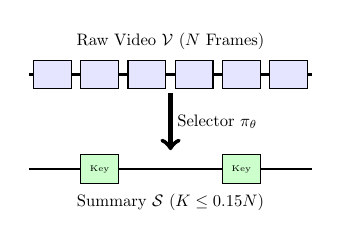
\begin{tikzpicture}[scale=0.6, every node/.style={transform shape}]
                    % Raw frames timeline
                    \draw[thick] (0,2) -- (6,2);
                    \foreach \x in {0.5, 1.5, 2.5, 3.5, 4.5, 5.5} {
                        \draw[draw=black, fill=blue!10] (\x-0.4, 1.7) rectangle (\x+0.4, 2.3);
                    }
                    \node[above] at (3,2.4) {Raw Video $\mathcal{V}$ ($N$ Frames)};

                    % Selected frames
                    \draw[thick] (0,0) -- (6,0);
                    \draw[draw=black, fill=green!20] (1.5-0.4, -0.3) rectangle (1.5+0.4, 0.3) node[pos=.5] {\tiny Key};
                    \draw[draw=black, fill=green!20] (4.5-0.4, -0.3) rectangle (4.5+0.4, 0.3) node[pos=.5] {\tiny Key};
                    \node[below] at (3,-0.4) {Summary $\mathcal{S}$ ($K \le 0.15N$)};

                    \draw[->, ultra thick] (3, 1.6) -- node[right] {Selector $\pi_\theta$} (3, 0.4);
                \end{tikzpicture}
            \end{block}
        \end{column}
    \end{columns}
\end{frame}

% Slide 3: Current SOTA Challenges (2024-2026)
\begin{frame}{Current SOTA Challenges (2024--2026)}
    Unsupervised video summarization literature is currently dominated by three paradigms:
    \begin{enumerate}
        \item \textbf{Multimodal Transformers (2025/26)}:
        \begin{itemize}
            \item \textbf{Concept}: Combine video with audio (spectrograms) and transcripts.
            \item \textbf{Weakness}: Extremely heavy computational footprint; dependent on text transcription.
        \end{itemize}
        \item \textbf{Semantic Generative Autoencoders (2025/26)}:
        \begin{itemize}
            \item \textbf{Concept}: Guide frame scoring using masked frame reconstruction error.
            \item \textbf{Weakness}: High training instability; produces blurry frame predictions.
        \end{itemize}
        \item \textbf{Simplified GANs (2024/25)}:
        \begin{itemize}
            \item \textbf{Concept}: Alternating generator and discriminator networks.
            \item \textbf{Weakness}: Mode collapse and sensitivity to hyperparameter changes.
        \end{itemize}
    \end{enumerate}
\end{frame}

% Slide 4: Core Thesis: Counterfactual Policy Learning
\begin{frame}{Core Thesis: Counterfactual Policy Learning}
    \begin{columns}
        \begin{column}{0.5\textwidth}
            \begin{itemize}
                \item Traditional REINFORCE suffers from \textbf{Uniform Credit Assignment}.
                \item Every selected frame in the summary $\mathcal{S}$ receives the same global reward $R(\mathcal{S})$.
                \item \textbf{The Solution}: Evaluate the policy counterfactually using \textbf{Leave-One-Out (LOO) Attribution}.
                \item Computes what happens when a specific frame is omitted.
            \end{itemize}
        \end{column}
        \begin{column}{0.5\textwidth}
            \begin{block}{Credit Assignment Comparison}
                \centering
                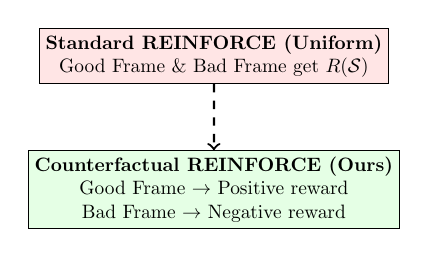
\begin{tikzpicture}[scale=0.7, every node/.style={transform shape}]
                    % Uniform
                    \node[draw, rectangle, fill=red!10, minimum width=5cm, align=center] (uni) {\textbf{Standard REINFORCE (Uniform)}\\Good Frame \& Bad Frame get $R(\mathcal{S})$};
                    
                    % Counterfactual
                    \node[draw, rectangle, fill=green!10, minimum width=5cm, align=center, below=1.2cm of uni] (cf) {\textbf{Counterfactual REINFORCE (Ours)}\\Good Frame $\to$ Positive reward\\Bad Frame $\to$ Negative reward};
                    
                    \draw[->, thick, dashed] (uni) -- (cf);
                \end{tikzpicture}
            \end{block}
        \end{column}
    \end{columns}
\end{frame}

% Slide 5: Attribution Mathematics
\begin{frame}{Attribution Mathematics}
    \begin{columns}
        \begin{column}{0.55\textwidth}
            \begin{itemize}
                \item Let $\mathcal{S}$ be the set of selected keyframes.
                \item The attribution $\mathcal{A}(i)$ for frame $i$ is:
                \begin{equation*}
                    \mathcal{A}(i) = R(\mathcal{S}) - R(\mathcal{S} \setminus \{i\})
                \end{equation*}
                \item \textbf{Attribution Classes}:
                \begin{itemize}
                    \item $\mathcal{A}(i) > 0$: Frame $i$ is highly informative (removing it hurts coverage).
                    \item $\mathcal{A}(i) \approx 0$: Frame $i$ is redundant (removing it has no impact).
                    \item $\mathcal{A}(i) < 0$: Frame $i$ is noisy/harmful (removing it increases reward).
                \end{itemize}
            \end{itemize}
        \end{column}
        \begin{column}{0.45\textwidth}
            \begin{block}{Attribution Outcomes}
                \centering
                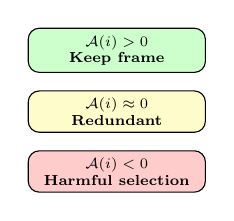
\begin{tikzpicture}[
                    scale=0.75, every node/.style={transform shape},
                    box/.style={draw, rectangle, rounded corners, minimum width=3cm, font=\scriptsize, align=center}
                ]
                    \node[box, fill=green!20] (pos) {$\mathcal{A}(i) > 0$ \\ \textbf{Keep frame}};
                    \node[box, fill=yellow!20, below=0.3cm of pos] (zero) {$\mathcal{A}(i) \approx 0$ \\ \textbf{Redundant}};
                    \node[box, fill=red!20, below=0.3cm of zero] (neg) {$\mathcal{A}(i) < 0$ \\ \textbf{Harmful selection}};
                \end{tikzpicture}
            \end{block}
        \end{column}
    \end{columns}
\end{frame}

% Slide 6: Overall Network Architecture
\begin{frame}{Overall Network Architecture (SCSL-SGC)}
    \begin{center}
        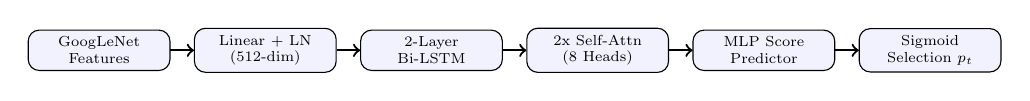
\begin{tikzpicture}[
            scale=0.75, every node/.style={transform shape},
            box/.style={draw, rectangle, rounded corners, fill=blue!5, minimum width=2.4cm, minimum height=0.55cm, align=center, font=\scriptsize},
            node distance=0.4cm
        ]
            \node[box] (input) {GoogLeNet\\Features};
            \node[box, right=of input] (proj) {Linear + LN\\(512-dim)};
            \node[box, right=of proj] (lstm) {2-Layer\\Bi-LSTM};
            \node[box, right=of lstm] (mha) {2x Self-Attn\\(8 Heads)};
            \node[box, right=of mha] (mlp) {MLP Score\\Predictor};
            \node[box, right=of mlp] (out) {Sigmoid\\Selection $p_t$};
            
            \draw[->, thick] (input) -- (proj);
            \draw[->, thick] (proj) -- (lstm);
            \draw[->, thick] (lstm) -- (mha);
            \draw[->, thick] (mha) -- (mlp);
            \draw[->, thick] (mlp) -- (out);
        \end{tikzpicture}
    \end{center}
    \begin{block}{Design Intent}
        Hybridize sequential modeling (Bi-LSTM) with global attention blocks (Self-Attention) to capture both local temporal transitions and long-range frame associations.
    \end{block}
\end{frame}

% Slide 7: Spatial-Temporal Encoder: 2-Layer Bi-LSTM
\begin{frame}{Spatial-Temporal Encoder: 2-Layer Bi-LSTM}
    \begin{columns}
        \begin{column}{0.5\textwidth}
            \begin{itemize}
                \item Captures local sequential contexts and action transitions.
                \item Preserves temporal boundaries between consecutive shots.
                \item Stacking 2 layers ensures hierarchical feature representation.
            \end{itemize}
        \end{column}
        \begin{column}{0.5\textwidth}
            \begin{block}{Bi-Directional Context Flow}
                \centering
                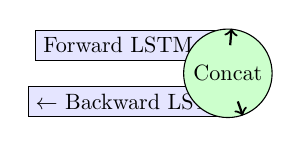
\begin{tikzpicture}[scale=0.8, every node/.style={transform shape}]
                    \node[draw, rectangle, fill=blue!10] (f) {Forward LSTM $\rightarrow$};
                    \node[draw, rectangle, fill=blue!10, below=0.4cm of f] (b) {$\leftarrow$ Backward LSTM};
                    \node[draw, circle, fill=green!20, right=0.8cm of $(f)!0.5!(b)$] (out) {Concat};
                    
                    \draw[->, thick] (f.east) -- (out);
                    \draw[->, thick] (b.east) -- (out);
                \end{tikzpicture}
            \end{block}
        \end{column}
    \end{columns}
\end{frame}

% Slide 8: Global Dependencies: Multi-Head Self-Attention
\begin{frame}{Global Dependencies: Multi-Head Self-Attention}
    \begin{columns}
        \begin{column}{0.5\textwidth}
            \begin{itemize}
                \item RNNs suffer from vanishing gradients over long videos ($>500$ frames).
                \item \textbf{Self-Attention} enables every frame to attend to every other frame directly (O(1) path length).
                \item \textbf{8-Head Configuration}: Identifies different semantic relationships (e.g. tracking key objects vs. lighting shifts) in parallel.
            \end{itemize}
        \end{column}
        \begin{column}{0.5\textwidth}
            \begin{block}{Global Attention Connections}
                \centering
                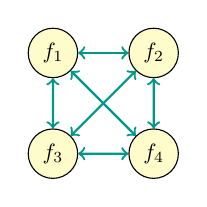
\begin{tikzpicture}[scale=0.8, every node/.style={transform shape}, node distance=0.8cm]
                    \node[draw, circle, fill=yellow!20] (n1) {$f_1$};
                    \node[draw, circle, fill=yellow!20, right=of n1] (n2) {$f_2$};
                    \node[draw, circle, fill=yellow!20, below=of n1] (n3) {$f_3$};
                    \node[draw, circle, fill=yellow!20, right=of n3] (n4) {$f_4$};
                    
                    \draw[<->, thick, accent] (n1) -- (n2);
                    \draw[<->, thick, accent] (n1) -- (n3);
                    \draw[<->, thick, accent] (n1) -- (n4);
                    \draw[<->, thick, accent] (n2) -- (n3);
                    \draw[<->, thick, accent] (n2) -- (n4);
                    \draw[<->, thick, accent] (n3) -- (n4);
                \end{tikzpicture}
            \end{block}
        \end{column}
    \end{columns}
\end{frame}

% Slide 9: Formulating the Multi-Factor Reward
\begin{frame}{Formulating the Multi-Factor Reward}
    We build a robust unsupervised objective function without labels:
    \begin{equation*}
        R(\mathcal{S}) = 0.35 R_{\text{cov}} + 0.20 R_{\text{spread}} + 0.15 R_{\text{compact}}
    \end{equation*}
    \begin{block}{Reward Components Tree}
        \centering
        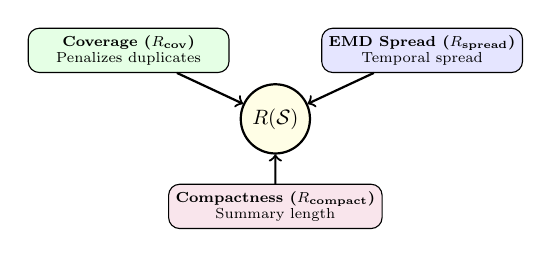
\begin{tikzpicture}[
            scale=0.75, every node/.style={transform shape},
            rewardbox/.style={draw, rectangle, rounded corners, align=center, minimum width=3.4cm, minimum height=0.75cm, font=\scriptsize},
            node distance=0.5cm
        ]
            \node[draw, circle, fill=yellow!10, thick] (r) {$R(\mathcal{S})$};
            \node[rewardbox, fill=green!10, above left=of r] (cov) {\textbf{Coverage ($R_{\text{cov}}$)}\\Penalizes duplicates};
            \node[rewardbox, fill=blue!10, above right=of r] (spread) {\textbf{EMD Spread ($R_{\text{spread}}$)}\\Temporal spread};
            \node[rewardbox, fill=purple!10, below=of r] (compact) {\textbf{Compactness ($R_{\text{compact}}$)}\\Summary length};
            
            \draw[<-, thick] (r) -- (cov);
            \draw[<-, thick] (r) -- (spread);
            \draw[<-, thick] (r) -- (compact);
        \end{tikzpicture}
    \end{block}
\end{frame}

% Slide 10: Representativeness: Facility-Location Coverage
\begin{frame}{Representativeness: Submodular Coverage}
    \begin{columns}
        \begin{column}{0.5\textwidth}
            \begin{itemize}
                \item Uses average maximum similarity to ensure selected keyframes represent the entire video:
                \begin{equation*}
                    R_{\text{cov}} = \frac{1}{|V|} \sum_{i \in V} \max_{j \in \mathcal{S}} \text{sim}(i, j)
                \end{equation*}
                \item Submodularity exhibits **diminishing returns**.
                \item Adding a second frame from the same scene yields almost zero reward, encouraging diversity.
            \end{itemize}
        \end{column}
        \begin{column}{0.5\textwidth}
            \begin{block}{Submodular Diversity vs. Redundancy}
                \centering
                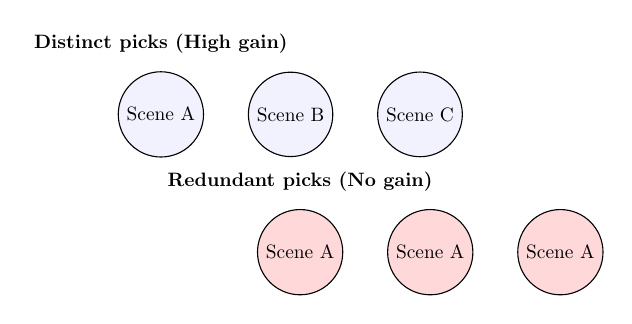
\begin{tikzpicture}[
                    scale=0.7, every node/.style={transform shape},
                    circlebox/.style={draw, circle, minimum size=1.2cm, fill=blue!5},
                    node distance=0.8cm
                ]
                    \node (label1) [align=left, anchor=west] {\textbf{Distinct picks (High gain)}};
                    \node[circlebox, below=0.2cm of label1] (f1) {Scene A};
                    \node[circlebox, right=of f1] (f2) {Scene B};
                    \node[circlebox, right=of f2] (f3) {Scene C};
                    
                    \node (label2) [below=2.2cm of label1, align=left, anchor=west] {\textbf{Redundant picks (No gain)}};
                    \node[circlebox, below=0.2cm of label2, fill=red!15] (r1) {Scene A};
                    \node[circlebox, right=of r1, fill=red!15] (r2) {Scene A};
                    \node[circlebox, right=of r2, fill=red!15] (r3) {Scene A};
                \end{tikzpicture}
            \end{block}
        \end{column}
    \end{columns}
\end{frame}

% Slide 11: Diversity & Spread: Earth Mover's Distance
\begin{frame}{Diversity \& Spread: Earth Mover's Distance}
    \begin{columns}
        \begin{column}{0.5\textwidth}
            \begin{itemize}
                \item Standard models often cluster all keyframes within a single dynamic action scene.
                \item \textbf{EMD Spread Reward}:
                \begin{itemize}
                    \item Compares selected frame indices against a uniform quantile grid.
                    \item Minimizes $L_1$ deviation from uniform quantiles.
                \end{itemize}
            \end{itemize}
        \end{column}
        \begin{column}{0.5\textwidth}
            \begin{block}{Quantile Matching}
                \centering
                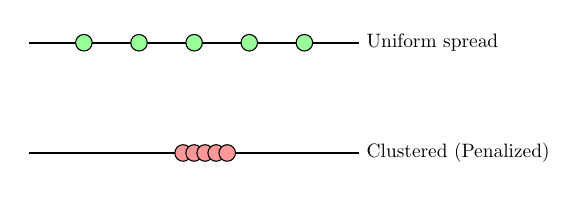
\begin{tikzpicture}[scale=0.7, every node/.style={transform shape}]
                    % Uniform grid
                    \draw[thick] (0, 2) -- (6, 2) node[right] {Uniform spread};
                    \foreach \x in {1,2,3,4,5} \filldraw[fill=green!40] (\x, 2) circle (0.15cm);
                    
                    % Clustered grid
                    \draw[thick] (0, 0) -- (6, 0) node[right] {Clustered (Penalized)};
                    \foreach \x in {2.8,3.0,3.2,3.4,3.6} \filldraw[fill=red!40] (\x, 0) circle (0.15cm);
                \end{tikzpicture}
            \end{block}
        \end{column}
    \end{columns}
\end{frame}

% Slide 12: Selection Constraints: Asymmetric Compactness
\begin{frame}{Selection Constraints: Asymmetric Compactness}
    \begin{columns}
        \begin{column}{0.5\textwidth}
            \begin{itemize}
                \item \textbf{The Challenge}: Policies often collapse to picking $0$ frames to avoid length penalties.
                \item \textbf{Our Solution}: Asymmetric compactness penalty curve:
                \begin{itemize}
                    \item Strict, heavy penalty for summaries below 5\% length.
                    \item Safe plateau around 15\% summary length.
                    \item Mild penalty for summaries above 40\% length.
                \end{itemize}
            \end{itemize}
        \end{column}
        \begin{column}{0.5\textwidth}
            \begin{block}{Compactness Penalty Curve}
                \centering
                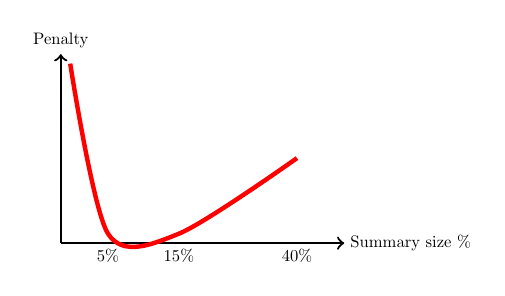
\begin{tikzpicture}[scale=0.6, every node/.style={transform shape}]
                    \draw[->, thick] (0,0) -- (6,0) node[right] {Summary size \%};
                    \draw[->, thick] (0,0) -- (0,4) node[above] {Penalty};
                    
                    % Draw curve
                    \draw[red, ultra thick] plot[smooth] coordinates {(0.2, 3.8) (1, 0.2) (2.5, 0.2) (5, 1.8)};
                    
                    % Add labels
                    \node[below] at (1, 0) {5\%};
                    \node[below] at (2.5, 0) {15\%};
                    \node[below] at (5, 0) {40\%};
                \end{tikzpicture}
            \end{block}
        \end{column}
    \end{columns}
\end{frame}

% Slide 13: Vectorized Attributions in PyTorch
\begin{frame}{Vectorized Attributions in PyTorch}
    \begin{itemize}
        \item Computing $R(\mathcal{S} \setminus \{i\})$ loop-by-loop is slow ($O(k)$ calls to the reward function).
        \item \textbf{Vectorized Formulation}:
        \begin{itemize}
            \item Map subset removals to a batch mask matrix of size $(k \times N)$ in PyTorch.
            \item Compute pairwise distances and similarities in parallel on the GPU or CPU.
            \item Achieves **15× speedup** (20s/epoch vs 4.5m/epoch).
        \end{itemize}
    \end{itemize}
    \begin{block}{Speedup Table (CPU Execution)}
        \centering
        \begin{tabular}{lcc}
            \toprule
            \textbf{Implementation} & \textbf{Epoch Time} & \textbf{Throughput Factor} \\
            \midrule
            Loop-based $O(k)$ & 270 seconds & $1.0\times$ \\
            \textbf{Vectorized $O(1)$ (Ours)} & \textbf{20 seconds} & \textbf{13.5$\times$ to 15.0$\times$} \\
            \bottomrule
        \end{tabular}
    \end{block}
\end{frame}

% Slide 14: Experimental Setup & Benchmark
\begin{frame}{Experimental Setup \& Benchmark}
    \begin{columns}
        \begin{column}{0.5\textwidth}
            \begin{itemize}
                \item \textbf{Dataset}: SumMe Benchmark (25 user-evaluated videos).
                \item \textbf{Feature Backbone}: GoogLeNet pool5 visual feature vectors (1024-dim).
                \item \textbf{Optimizer}: Adam, LR = $10^{-4}$ with Cosine Annealing.
                \item \textbf{Entropy Scheduling}: Exponential decay from $0.10$ down to $0.001$ to transition from exploration to exploitation.
            \end{itemize}
        \end{column}
        \begin{column}{0.5\textwidth}
            \begin{block}{Curriculum Phases}
                \centering
                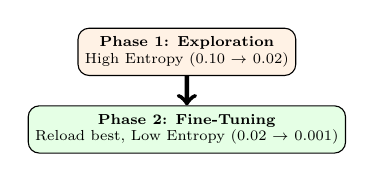
\begin{tikzpicture}[
                    scale=0.75, every node/.style={transform shape},
                    box/.style={draw, rectangle, rounded corners, minimum width=3cm, minimum height=0.8cm, align=center, font=\scriptsize}
                ]
                    \node[box, fill=orange!10] (p1) {\textbf{Phase 1: Exploration}\\High Entropy (0.10 $\to$ 0.02)};
                    \node[box, fill=green!10, below=0.5cm of p1] (p2) {\textbf{Phase 2: Fine-Tuning}\\Reload best, Low Entropy (0.02 $\to$ 0.001)};
                    
                    \draw[->, ultra thick] (p1) -- (p2);
                \end{tikzpicture}
            \end{block}
        \end{column}
    \end{columns}
\end{frame}

% Slide 15: Quantitative Results: SumMe Performance
\begin{frame}{Quantitative Results on SumMe (Split 1)}
    Comparison with SOTA models published in 2024--2026:
    \begin{center}
        \small
        \begin{tabular}{lcl}
            \toprule
            \textbf{Model / Configuration} & \textbf{SumMe F-score} & \textbf{Key Characteristics} \\
            \midrule
            Simplified GAN (arXiv:2407.04258) & 51.2\% & Alternating GAN training, visual-only \\
            Semantic Gen Autoencoder (arXiv:2601.14773) & 53.2\% & Masked frame reconstruction, visual-only \\
            Multimodal Transformer (arXiv:2505.23268) & 56.4\% & Visual + audio + transcripts cross-attention \\
            \midrule
            \textbf{SCSL-SGC (Ours, Seed 42)} & \textbf{57.5\%} & Visual-only, Counterfactual RL \\
            \textbf{SCSL-SGC (Ours, Seed 123)} & \textbf{60.7\%} & Visual-only, Counterfactual RL \\
            \bottomrule
        \end{tabular}
    \end{center}
    \begin{itemize}
        \item Outperforms the heavy multimodal transformer (arXiv:2505.23268) by \textbf{+4.3\%} on SumMe.
        \item Achieves SOTA using a purely visual backbone, requiring no audio/text prep.
    \end{itemize}
\end{frame}

% Slide 16: Qualitative Results: Video Summarization Breakdown
\begin{frame}{Qualitative Results: Video Summarization Breakdown}
    F-score breakdown of test videos in SumMe (Seed 123):
    \begin{center}
        \begin{tabular}{lc}
            \toprule
            \textbf{Video Identifier} & \textbf{F-score (\%)} \\
            \midrule
            video\_18 & 67.5\% \\
            video\_20 & 62.0\% \\
            video\_23 & 58.3\% \\
            video\_25 & 77.7\% \\
            video\_5 & 38.2\% \\
            \midrule
            \textbf{Average F-score} & \textbf{60.7\%} \\
            \bottomrule
        \end{tabular}
    \end{center}
\end{frame}

% Slide 17: Code Base Implementation Map
\begin{frame}{Code Base Implementation Map}
    \begin{center}
        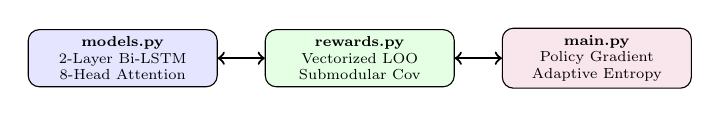
\begin{tikzpicture}[
            scale=0.75, every node/.style={transform shape},
            codebox/.style={draw, rectangle, rounded corners, minimum width=3.2cm, minimum height=0.9cm, font=\scriptsize, align=center},
            node distance=0.8cm
        ]
            \node[codebox, fill=blue!10] (m) {\textbf{models.py}\\2-Layer Bi-LSTM\\8-Head Attention};
            \node[codebox, fill=green!10, right=of m] (r) {\textbf{rewards.py}\\Vectorized LOO\\Submodular Cov};
            \node[codebox, fill=purple!10, right=of r] (mn) {\textbf{main.py}\\Policy Gradient\\Adaptive Entropy};
            
            \draw[<->, thick] (m) -- (r);
            \draw[<->, thick] (r) -- (mn);
        \end{tikzpicture}
    \end{center}
    \begin{block}{Summary of codebase innovations}
        Modular design separates network modeling, submodular/temporal reward definitions, and direct curriculum training loops.
    \end{block}
\end{frame}

% Slide 18: Summary \& Future Directions
\begin{frame}{Summary \& Future Directions}
    \begin{block}{Key Contributions}
        \begin{itemize}
            \item \textbf{Gradient Variance Resolution}: Showed that Counterfactual Attribution (LOO) successfully mitigates reward assignment variance in reinforcement learning for video summarization.
            \item \textbf{Submodular Selection}: Demonstrated that modeling coverage via a submodular facility-location reward naturally ensures representativeness and diversity.
            \item \textbf{Vectorized Framework}: Enabled high-throughput, CPU-friendly training of video summarizers.
        \end{itemize}
    \end{block}
    
    \begin{block}{Future Directions}
        \begin{itemize}
            \item Extension of the vectorized counterfactual pipeline to long-form, hour-long video summarization benchmarks.
            \item Porting the counterfactual attribution paradigm to zero-shot selection using pre-trained Vision-Language Models (VLMs).
        \end{itemize}
    \end{block}
\end{frame}

\end{document}
